\chapter{PROLOG}

Sudah hampir 200 tahun setelah perang dunia ke-tiga menghancurkan 1/3 dunia. Kegilaan itu berhasil menghilangkan 60\% spesies makhluk hidup yang ada kala itu. Namun perdamaian dunia menggagalkan kelanjutan perang tersebut dan memberikan pandangan baru kepada dunia. Inofasi energi masal selain nuklir telah ditemukan kala berakhirnya kegilaan yang dahulu. Sebuah gedung riset pabrik senjata meledak dan menghancurkan 1/3 dunia. Jika perang dunia berakhir karena telah terjadi ledakan rudal(nuklir), namun kali ini karena kegagalan pembuatan rudal tipe terbaru. Kini perdamaian dunia terjalin, sisi terang dunia sudah mulai berinar bersinar lagi. Namun semakin terang cahaya yang bersinar akan semakin gelap bayangannya.

Terbangun aku dimalam hari. Dingin angin malam berhembus membuatku menggigil. Suara raungan perut kosong meramaikan kamar kecil yang hanya seukuran 2x2 tinggi manusia dewasa rata-rata. Di sisi terang dunia aku tinggal di balik bayangannya. Hanya mengenakan kaos dan celana pendek aku duduk termenung melihat langit dari jendela sembari menggam mouse PC di tangan kanan. Biarpun ku menatap langit yang hanya bisa aku lihat hanyalah awan tebal merah dengan kabut asap. Bintang bintang yang aku berasal dari tiang tiang dan tembok tembok raksasa menjulang tinggi kelangit. Ku palingkan pandangan ku ke PC tua yang sudah usang dan berdebu ini. Hampir se-abad PC tua ini digunakan turun temurun. Aku mulai merapihkan data yang sudah terkumpul tadi siang kedalam kelas dan katagori. Data yang ku kumpulkan adalah data tentang tanaman dan makhluk hidup lainnya yang masih hidup di sekitar sini dan cara untuk membudidayakannya. Ya, termasuk membudidayakan rumput dan kutu. Ku kumpulkan semua data itu setiap hari dan merangkumnya dalam sebuah database ensiklopedia yang aku terbitkan dalam artikel majalah elektronik lokal setiap minggunya. Pendapatan dari terbitan itu cukup untuk aku makan 5 hari. Tidak hanya data tentang makhluk hidup yang aku kumpulkan, semua informasi baik itu dari teknologi terbaru dan canggih hingga tetangga yang ketauan selingkuh aku kumpulkan. Namun aku tak akan mempublikasikan informasi sosial dan provokatif. Kau tau aturan negara ini, bila kau kedapatan melakukannya maka kehadiranmu akan hilang dari sejarah. Kau tahu maksudku.

\clearpage
\tikz[remember picture,overlay] \node[opacity=1.0,inner sep=0pt] at (current page.center){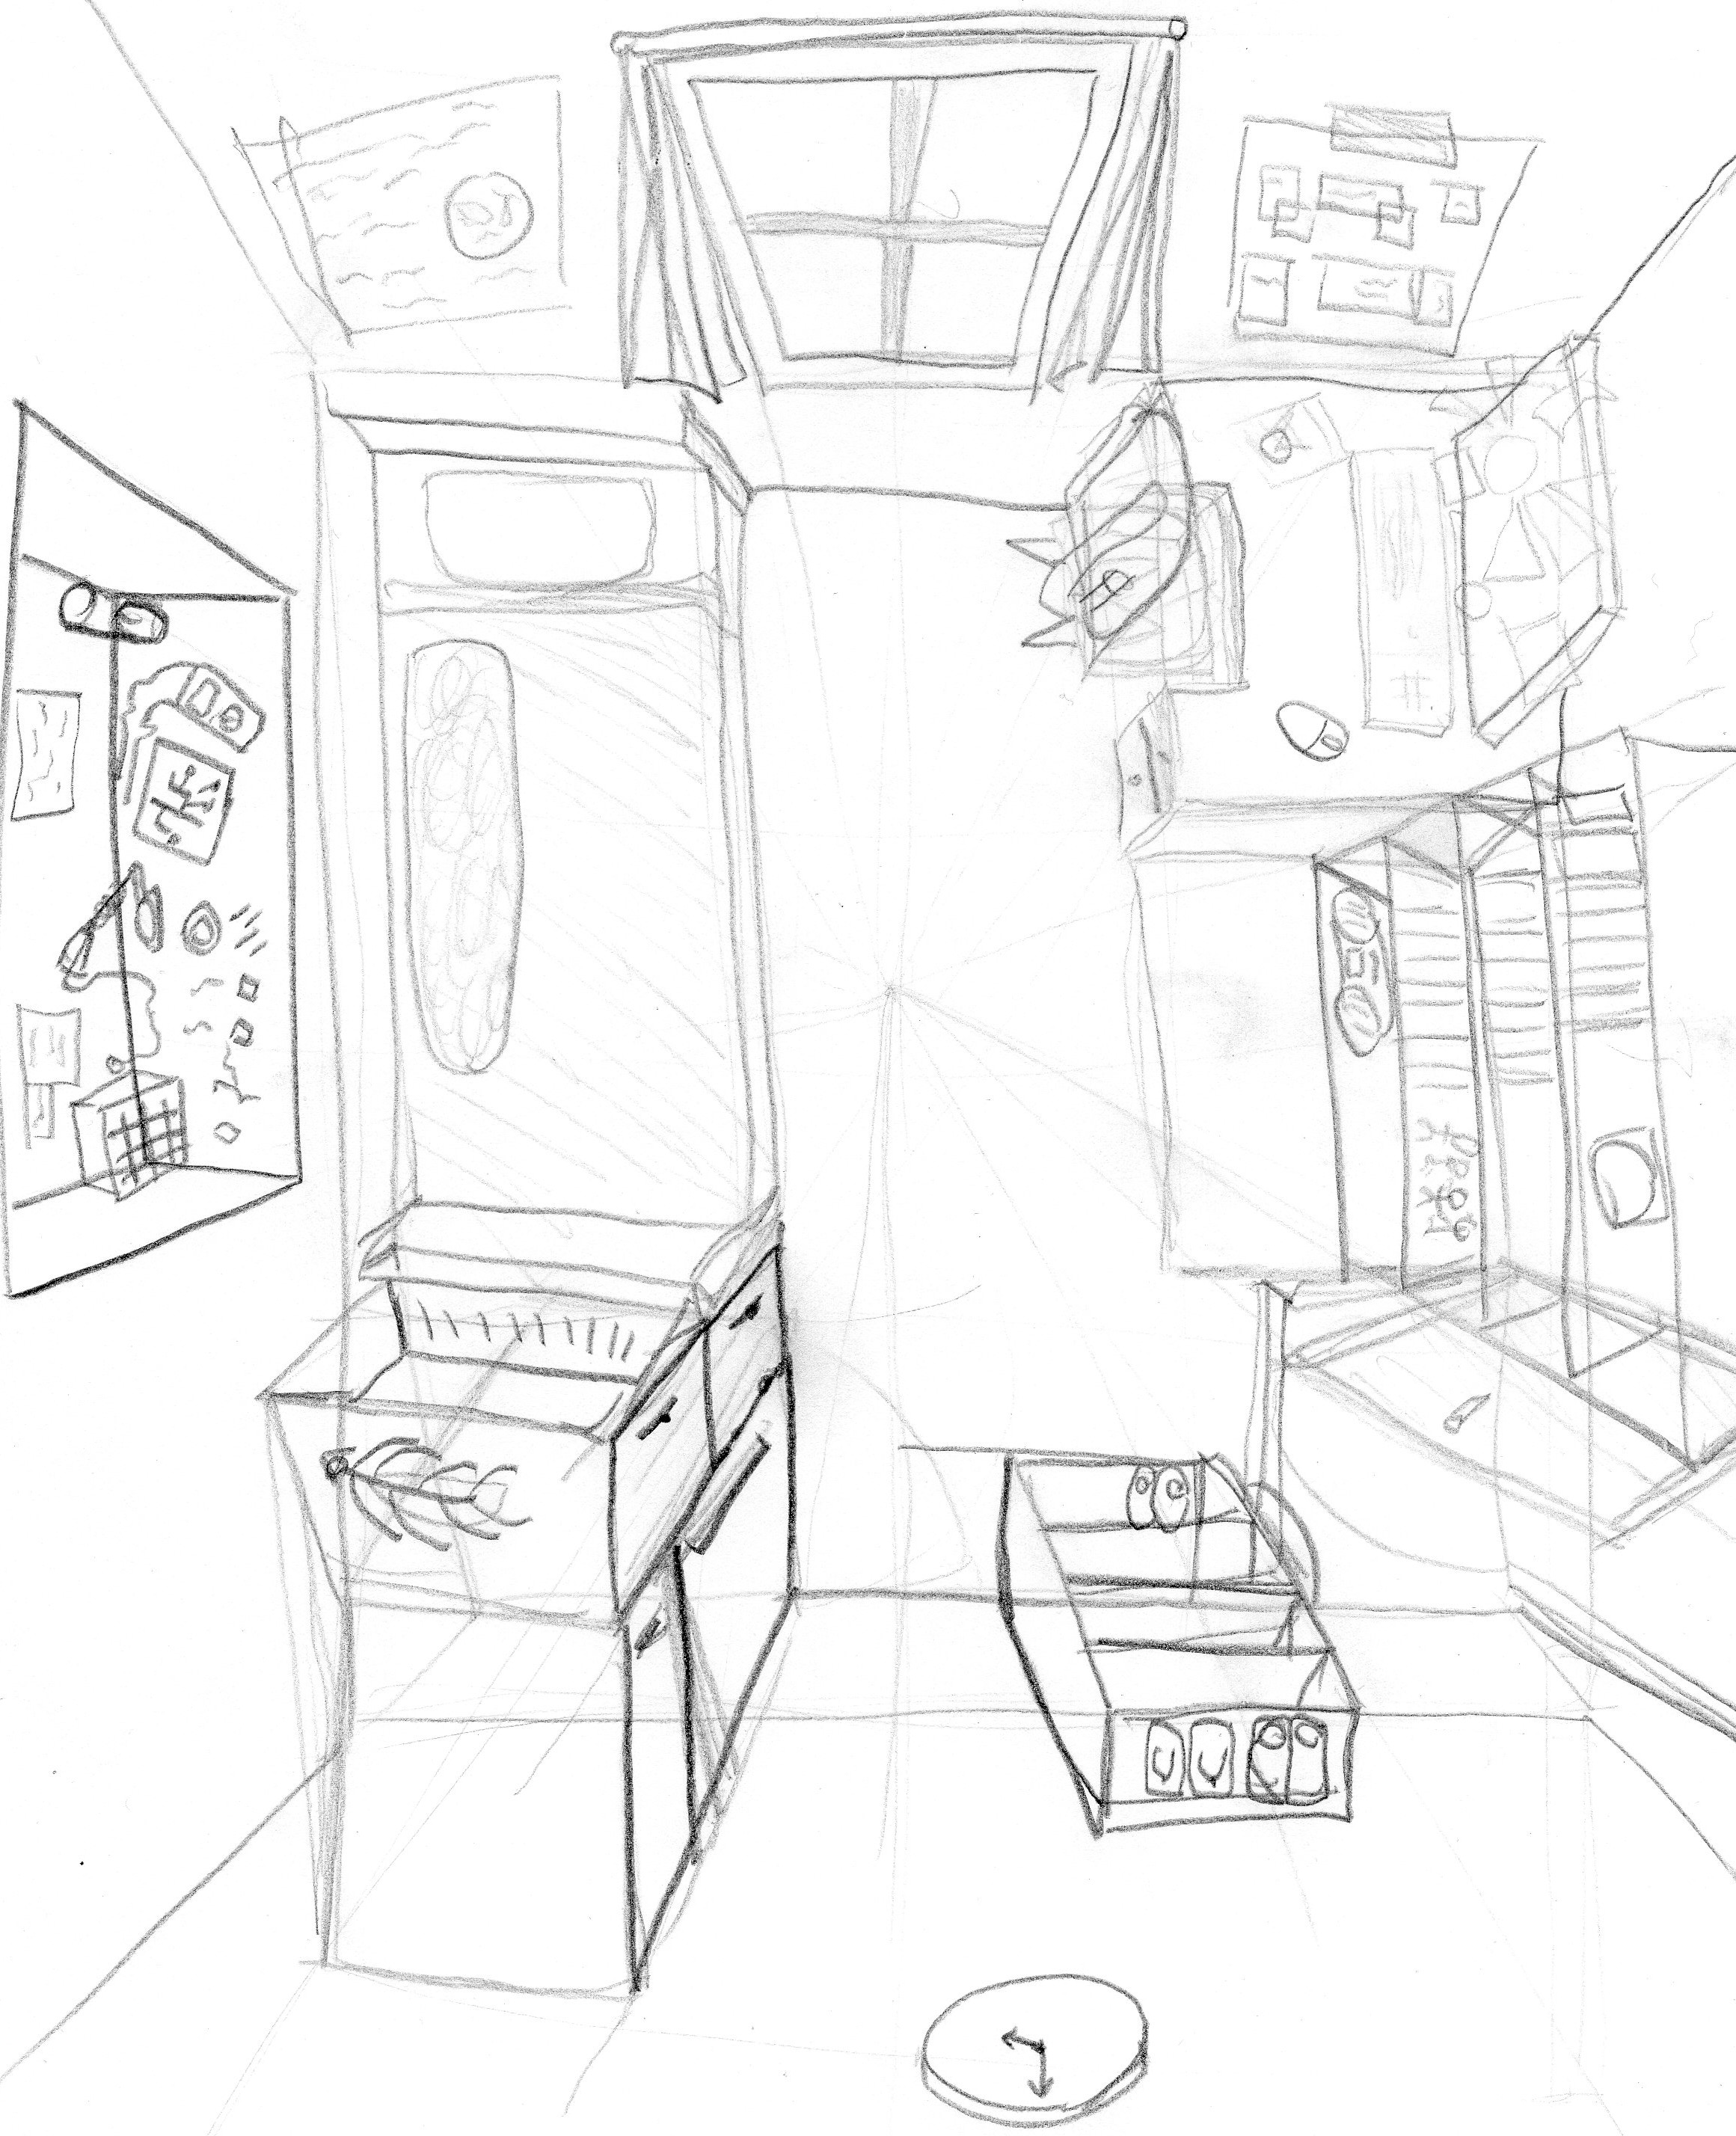
\includegraphics[width=\paperwidth,height=\paperheight]{./images/0}};